\chapter{Forces}

\section*{LEARNING OUTCOMES}
{
\begin{center}
\fcolorbox{black}{shadecolor}{%

    \parbox{0.95\textwidth}
    {%
        \small
        {
        \begin{itemize}[leftmargin=*]\itemsep0em
            \item What is a force? What does it mean according to physics?
            \item What can force do (moving and stopping objects etc.)?
            \end{itemize}
        }
    }%
}
\end{center}
}

\section*{DEMONSTRATIONS}
\section*{Measurement of Pressure via Piezoelectric Sensor}
For this experiment, you will need:

\begin{table}[H]
    \centering
    \begin{tabular}{|c|l|c|}\hline
     \textbf{\#} & \textbf{Components}  &  \textbf{Amount}\\\hline
     1 & LED                            &  1\\\hline
     2 & 1 M$\Omega$ resistor           & 1\\\hline
     3 & 470 $\Omega$ resistor           & 1\\\hline
     4 & Piezoelectric sensor                   &  1\\\hline
     5 & Breadboard                     & 1\\\hline
     6 & Arduino microcontroller board  &  1\\\hline
     7 & Connecting wires               & - \\\hline
    \end{tabular}
\end{table}

\subsection*{Connections}
\begin{enumerate}[leftmargin=*]
    \item Connect the GND terminal of the piezoelectric sensor to the GND pin of Arduino by using a breadboard. Connect its POSITIVE terminal with pin A$0$.
    \item Connect a 1 M$\Omega$ resistor between the terminals of the piezoelectric sensor.
    \item Connect the anode of the LED to pin 9 through a 470 $\Omega$ resistor. Connect the cathode of the LED directly to GND terminal.
\end{enumerate}

\begin{figure}[H]
    \centering
    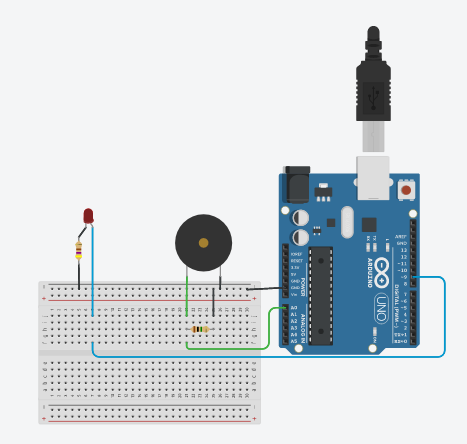
\includegraphics[scale=0.7]{Figures/force.PNG}
    \caption{Circuit diagram}
\end{figure}

\subsection*{Procedure}
\begin{enumerate}[leftmargin=*]
    \item Copy lst. \ref{lst:force} to a new Arduino sketchbook. Upload the code to your Arduino board. Also open the Serial Monitor.
    \item Press the piezoelectric sensor and observe the change in the state of LED.
\end{enumerate}

\begin{lstlisting}[language=Arduino, numbers=none, caption={Arduino code for measuring the pressure},captionpos=b, label={lst:force}]

int pressure;           // stores the pressure reading 
int pressurePin=A0;     // pin A0 reads the pressure
int ledPin=9;           // pin 9 controls the LED

void setup() 
{
  pinMode(pressurePin, INPUT);   //configure A0 as input pin
  pinMode(ledPin, OUTPUT);      //configure pin5 as output pin
  Serial.begin(9600);           //set the baud rate to be 9600
 }// void setup ends here

void loop() 
{
  // Measure the pressure reading from pin A0
  pressure = analogRead(pressurePin);
  
  // Print the temperature reading on the screen
  Serial.println("Pressure= ");
  Serial.print(pressure);

  analogWrite(ledPin, pressure/4);
  
  // Wait for 1 sec before the next reading
  delay(100);
}// loop ends here

\end{lstlisting}

\begin{figure}[H]
    \centering
    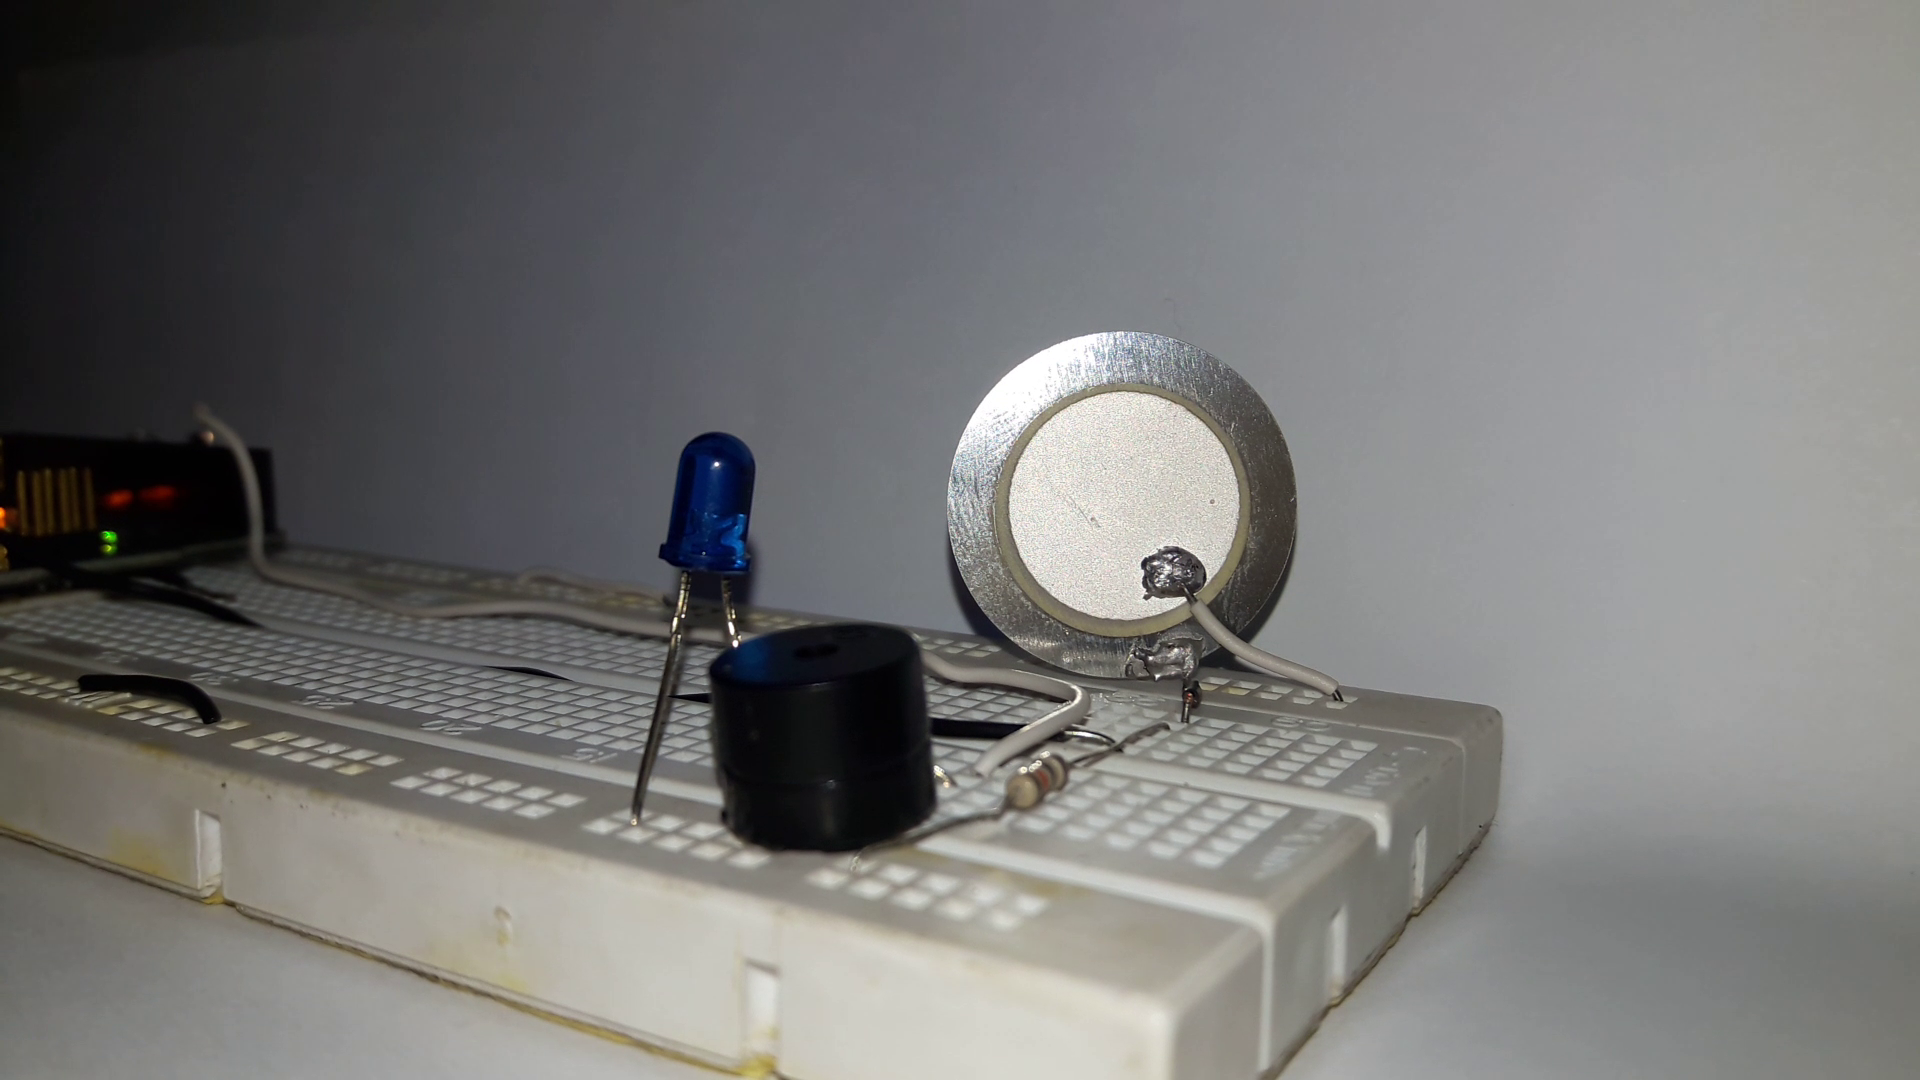
\includegraphics[width=0.75\linewidth]{Figures/force-hardware.png}
    \caption{Hardware of the experiment}
\end{figure}

\subsection*{Precautions}
Touch the piezoelectric sensor gently. Coarse handling may loosen the connections and affect the measurements.